\subsection{Ebenen des Testing \hfill IP}
    \begin{scriptsize}
        \begin{itemize}
            \item \textbf{Verifizierung:} Prüfstand oder Nutzer / klare Fragestellung / Funktion testen \\$\to$ \textbf{nicht} Bauteile / Testfälle und Zielparameter
            \item \textbf{Validierung:} Nutzer und reale Anwendung / Vergleich Kundenbedürfnis zu System-\\verhalten / Gesamtnutzen testen / Anwendung auch auf unvorhergesehene Weise
            \item \textbf{Ausprobieren:} Zusammenhänge verstehen / Verständnis, Gefühle entwickeln \\/ Inspiration für neue Ideen
            \item \textbf{Experiment:} Bestätigung od. Widerlegung Hypothesen / Ermittlung der Einfluss-\\parameter / Entwicklung von Modellen
            \item \textbf{Verifikation:} Überprüfung einer Zielgrösse / Absicherung von Anforderungen \\/ Eindeutige Erfüllungskriterien (Ja / Nein)
            \item \textbf{Validierung:} Testen in der Anwendung mit Nutzer / Absicherung eines robusten \\ Systems / Ermittlung von unbekannten Effekten
        \end{itemize}
        \centering{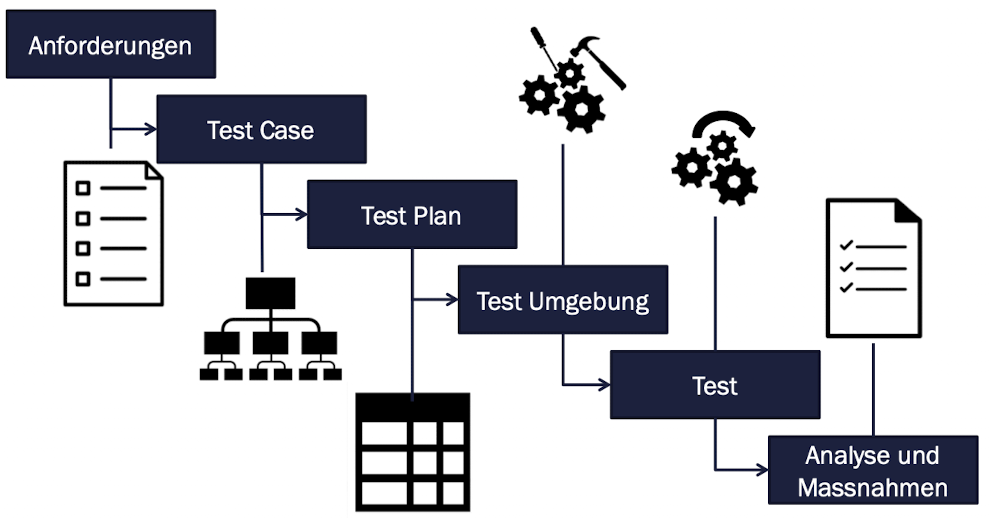
\includegraphics[width = 0.6\linewidth]{src/images/MAEIP_Testing_2}}
    \end{scriptsize}